% VUT FIT MITAI
% PRL 2019/2020
% Project 2: Odd-even transposition sort algorithm
% Author: Vladimir Dusek
% Login: xdusek27

%%%%%%%%%%%%%%%%%%%%%%%%%%%%%%%%%%%%%%%%%%%%%%%%%%%%%%%%%%%%%%%%%%%%%

\documentclass[11pt, a4paper, titlepage]{article}
\usepackage[left=2cm, text={17cm, 24cm}, top=3cm]{geometry}
\usepackage[utf8]{inputenc}
\usepackage[czech]{babel}
\usepackage{pdfpages}
\usepackage[T1]{fontenc}
\usepackage{amsmath}
\usepackage{graphicx}
\usepackage{float}

\begin{document}

%%%%%%%%%%%%%%%%%%%%%%%%%%%%%%%%%%%%%%%%%%%%%%%%%%%%%%%%%%%%%%%%%%%%%

\begin{center}
    \Large Paralelní a distribuované algoritmy (PRL)
    \bigskip

    \Large Dokumentace k~$2.$ projektu: \textit{Odd even transposition sort}
    \bigskip

    \Large Vladimír Dušek, xdusek27
    \bigskip
\end{center}

%%%%%%%%%%%%%%%%%%%%%%%%%%%%%%%%%%%%%%%%%%%%%%%%%%%%%%%%%%%%%%%%%%%%%

\section{Popis algoritmu}\label{sec:popis}

\textit{Odd even transposition sort} je řadící algoritmus.
Jedná se o~paralelní verzi známého sekvenčního algoritmu \textit{Bubble sort}.
Ten je jednoduchý na implementaci, avšak velice neefektivní.
Jedná se o~jeden z~nejpomalejších algoritmů, jeho časová asymptotická složitost je $O(n^2)$.
Je však pomalejší i v~porovnání s~jinými algoritmy se stejnou složitostí, neboť jeho primitivní implementace vyžaduje velké množství zápisů do paměti.

Algoritmus \textit{Odd even transposition sort} využívá toho, že porovnávání jednotlivých dvojic prvků je nezávislé na ostatních.
Paralelizace je tedy velmi jednoduchá a nevyžaduje žádnou speciální režii.
Funguje následujícím způsobem:

\begin{enumerate}
    \item Mějme lineární pole $n$ procesorů, kde $n$ je počet řazených prvků.
    \item Každý procesor $p_i$ se stará o~jednu z~řazených hodnot $y_i$.
    \item Každý lichý procesor $p_i$, kde $i = 1, \dots, n-1$, se spojí se svým pravým sousedem $p_{i+1}$ a porovnají své hodnoty.
          Je-li $y_i > y_{i+1}$, procesory vymění své hodnoty.
    \item Každý sudý procesor $p_i$, kde $i = 1, \dots, n-1$, se spojí se svým pravým sousedem $p_{i+1}$ a porovnají své hodnoty.
          Je-li $y_i > y_{i+1}$, procesory vymění své hodnoty.
    \item Fáze $3$ a $4$ se opakují, po maximálně $n$ opakováních jsou prvky seřazeny.
\end{enumerate}

Je zřejmé, že algoritmus se v~podstatě neliší od sekvenčního \textit{Bubble sort}.
Je pouze třeba nahradit sekvenční cykly za paralelní a průběh rozdělit na dvě podfáze, pro sudé a liché procesory.

%%%%%%%%%%%%%%%%%%%%%%%%%%%%%%%%%%%%%%%%%%%%%%%%%%%%%%%%%%%%%%%%%%%%%

\section{Rozbor algoritmu}\label{sec:rozbor}

\begin{itemize}
    \item Počet procesorů lineárně stoupá s~velikostí instance úlohy, tedy $p(n) = n$.
    \item Kroky $1$ a $2$ provádí jedno porovnání a dva přenosy, to nás stojí konstantní čas.
          Zbytek algoritmu pak probíhá v~jednom cyklu, kde probíhá porovnávání a přiřazování.
          Pokud zanedbáme multiplikativní a aditivní konstanty získáme celkově lineární časovou složitost $O(n)$.
    \item Algoritmus pouze prohazuje hodnoty ve dvojicích, žádná data si dále neukládá.
          Paměťové nároky se tak v~závislosti na velikosti vstupních dat nemění.
          Prostorová složitost algoritmu je tedy konstantní $O(1)$.
    \item Celková cena paralelního řešení je obecně definována jako $c(n) = p(n) \cdot t(n)$.
          V~našem případě tedy $c(n) = n \cdot O(n) = O(n^2)$.
    \item Algoritmus je optimální, pokud je jeho celková cena stejná jako časová složitost optimálního sekvenčního algoritmu.
    Ta činí $O(n \cdot \log(n))$.
    Je zřejmé, že $O(n \cdot \log(n)) < O(n^2)$, a proto \textit{Odd even transposition sort} není optimální.
    Aditivní a multiplikativní konstanty zanedbáváme.
\end{itemize}

%%%%%%%%%%%%%%%%%%%%%%%%%%%%%%%%%%%%%%%%%%%%%%%%%%%%%%%%%%%%%%%%%%%%%

\section{Popis implementace}\label{sec:implementace}

Aplikace je napsaná v~jazyce C/C++ s~využitím knihovny Open MPI pro paralelizaci.
Na vstup dostane soubor s~čísly, které je třeba seřadit.
Nejprve proběhne inicializace MPI a každý procesor zjistí svůj rank (id).
Master procesor (procesor s~rankem 0) otevře vstupní soubor, postupně čísla čte, vypisuje je na standardní výstup oddělené mezerou a posílá jednotlivým procesorům.
Každý procesor obdrží právě jedno číslo.

Jsou spočítány limity pro řazení, a sice celkový počet iterací jako $n/2$, kde $n$ je počet hodnot k~seřazení.
Limit pro liché fáze jako $2 \cdot (n/2) - 1$ a pro sudé $2 \cdot ((n - 1) / 2)$.
Ve smyčce se pak střídají sudé a liché fáze tak, jak bylo popsáno v~sekci~\ref{sec:rozbor}.
V~liché fázi, každý lichý procesor pošle své číslo svému pravému sousedovi (procesoru s~rankem vyšším o~1).
Soused (sudý procesor) obdrží sousedovu hodnotu, porovná ji se svojí a sousedovi vrátí nižší z~nich.
V~sudé fázi, každý sudý procesor pošle své číslo svému pravému sousedovi, ten udělá totéž jako v~liché fázi.
Po skončení smyčky jsou prvky seřazeny, respektive procesor s~rankem $0$ má nejnižší hodnotu a procesor s~rankem $n-1$ největší.

Nyní když jsou hodnoty seřazeny, je třeba je korektně vypsat na standardní výstup.
Abychom nemuseli řešit synchronizaci, je nutné, aby je vypisoval pouze jeden procesor.
Master procesor tedy vytvoří pole velikosti $n$.
Všechny ostatní procesory mu své hodnoty postupně pošlou a master procesor je uloží do pole.
Na konci postupně hodnoty vypíše a oddělí novým řádkem.

Pro otestování implementace je přiložen shell skript \texttt{test.sh}.
Ten pomocí unixové utility \texttt{dd} vygeneruje náhodná čísla veliká 1 byte a uloží je do souboru.
Následně přeloží zdrojový kód aplikace a spustí ji s~vygenerovaným souborem s~náhodnými čísly.
Nakonec veškeré vygenerované soubory smaže.

%%%%%%%%%%%%%%%%%%%%%%%%%%%%%%%%%%%%%%%%%%%%%%%%%%%%%%%%%%%%%%%%%%%%%

\section{Komunikační protokol}\label{sec:protokol}

\begin{figure}[H]
    \centering
    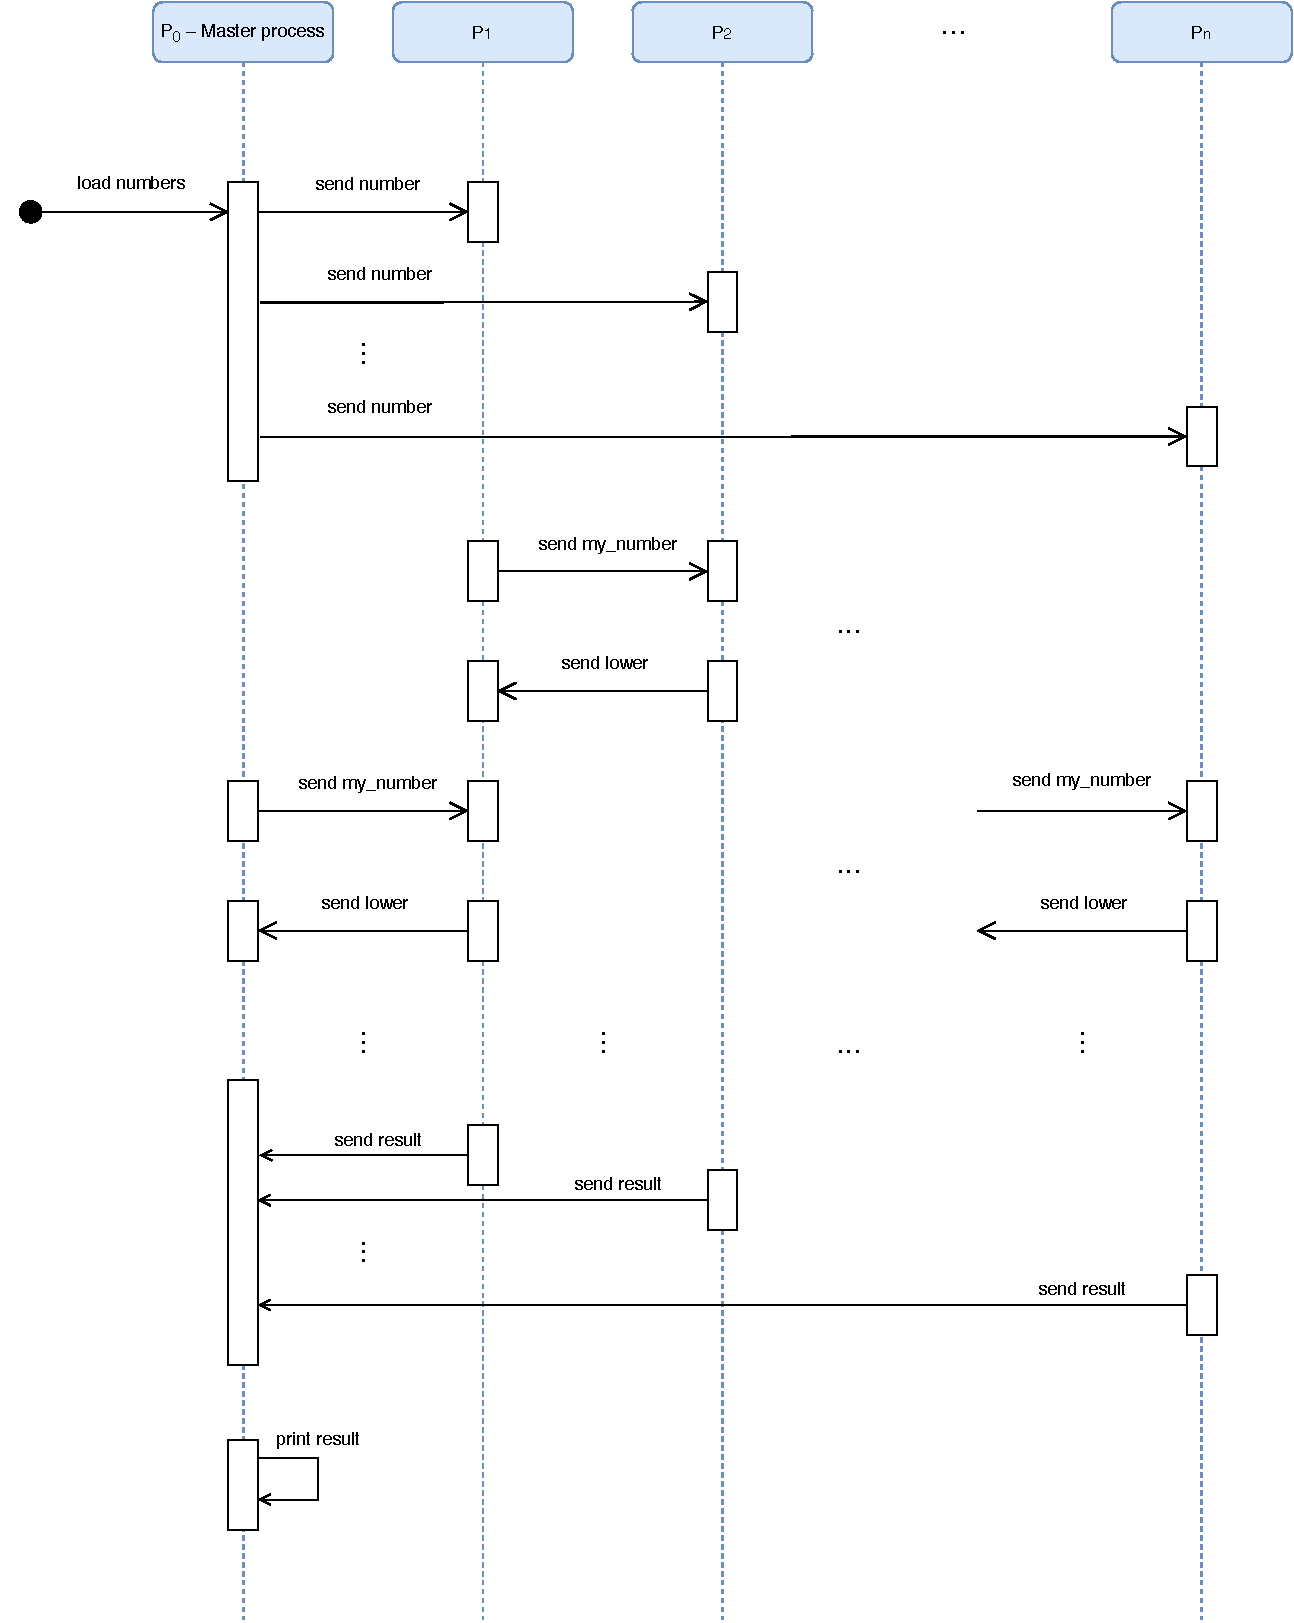
\includegraphics[width=.95\textwidth]{diagram.pdf}
    \caption{Komunikační protokol aplikace zakreslený sekvenčním diagramem.}
\end{figure}

%%%%%%%%%%%%%%%%%%%%%%%%%%%%%%%%%%%%%%%%%%%%%%%%%%%%%%%%%%%%%%%%%%%%%

\section{Experimenty pro ověření časové složitosti}\label{sec:experimenty}

Cílem experimentu bylo ověřit časovou složitost implementace \texttt{Odd even transposition sort} algoritmu.
Na školním serveru Merlin, kde byly experimenty prováděny, je možné spustit maximálně 25 procesů.
Vzhledem k~vlastnostem algoritmu, kdy počet procesů roste lineárně s~počtem hodnot, museli být experimenty prováděny pouze na počtu hodnot 2--25.

Měřeno bylo pouze samotné řazení, veškerá režie s~algoritmem spojená (čtení hodnot ze souboru, inicializace MPI, distribuce hodnot mezi procesy, vypisování, \ldots) nebyla brána v~potaz.
Pomocí funkce \texttt{MPI\_Wtime()} byl změřen čas běhu řadící smyčky.
Pro každou velikost množiny hodnot bylo provedeno 29 měření.
Byly vyřazena 2 nejvyšší a 2 nejnižší hodnoty, zbylých 25 hodnot bylo zprůměrováno.
Tím byl zjištěn čas řazení konkrétního počtu prvků.
\medskip

\begin{table}[H]

    \begin{tabular}{|l|p{1.25cm}p{1.25cm}p{1.25cm}p{1.25cm}p{1.25cm}p{1.25cm}p{1.25cm}p{1.25cm}p{1.25cm}|}
        \hline
        n             & 2     & 3     & 4     & 5     & 6     & 7     & 8     & 9      & 10     \\ \hline
        time {[}ns{]} & 13863 & 13148 & 42102 & 42129 & 48337 & 59587 & 89309 & 220289 & 190893 \\ \hline
    \end{tabular}
    \medskip

    \begin{tabular}{|l|p{1.25cm}p{1.25cm}p{1.25cm}p{1.25cm}p{1.25cm}p{1.25cm}p{1.25cm}p{1.25cm}p{1.25cm}|}
        \hline
        n             & 11     & 12     & 13     & 14     & 15     & 16     & 17     & 18     & 19     \\ \hline
        time {[}ns{]} & 168500 & 267072 & 276954 & 433162 & 457083 & 456730 & 507875 & 714275 & 923916 \\ \hline
    \end{tabular}
    \medskip

    \begin{tabular}{|l|p{1.25cm}p{1.25cm}p{1.25cm}p{1.25cm}p{1.25cm}p{1.25cm}|}
        \hline
        n             & 20     & 21      & 22      & 23      & 24      & 25      \\ \hline
        time {[}ns{]} & 815223 & 1016009 & 1211453 & 1213332 & 1397229 & 1453920 \\ \hline
    \end{tabular}
    \caption{Délka trvání řazení v~závislosti na počtu prvků.}
\end{table}

\begin{figure}[H]
    \centering
    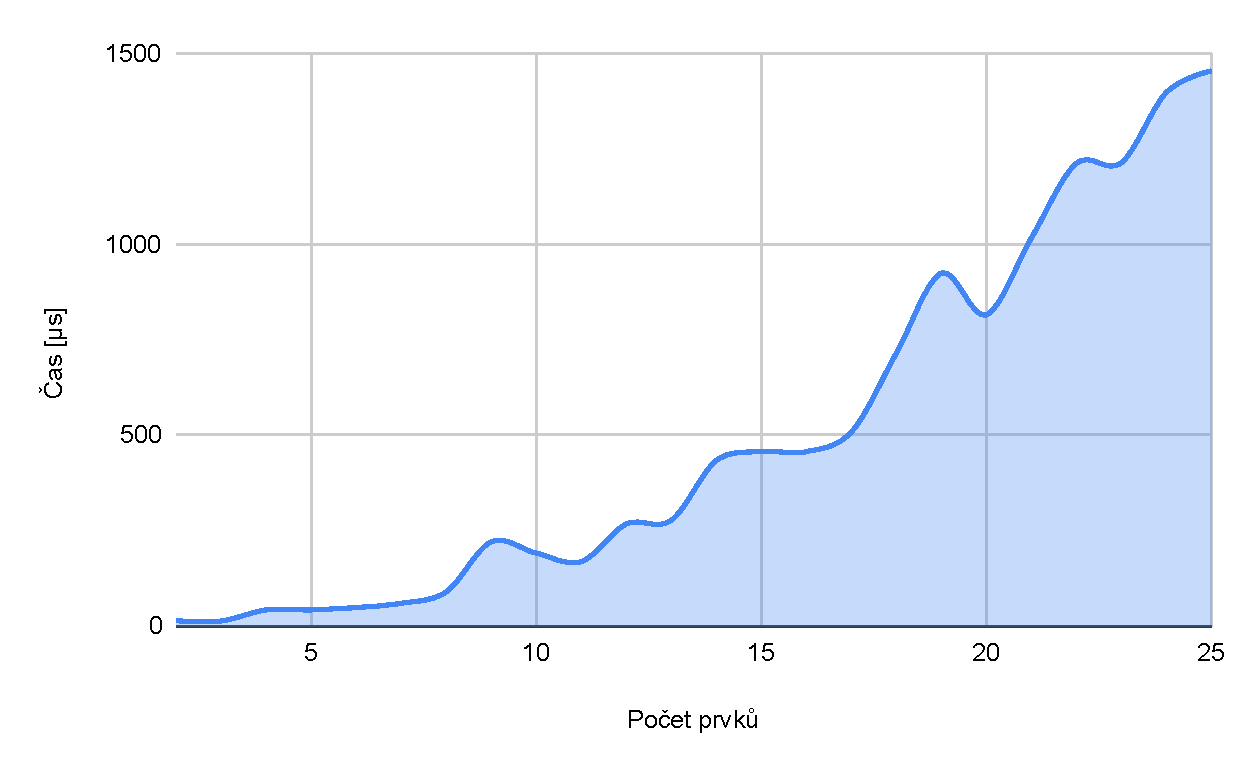
\includegraphics[width=.8\textwidth]{chart.pdf}
    \caption{Délka trvání řazení v~závislosti na počtu prvků.}
\end{figure}

%%%%%%%%%%%%%%%%%%%%%%%%%%%%%%%%%%%%%%%%%%%%%%%%%%%%%%%%%%%%%%%%%%%%%

\section{Závěr}\label{sec:zaver}

Výsledky měření v~kapitole~\ref{sec:experimenty} ukazují, že čas potřebný k~seřazení množiny prvků roste lineárně s~její mohutností.
Drobné výkyvy při měření lze dát za vinu různému zatížení školského serveru Merlin v~čase kdy probíhaly experimenty.
Toto zjištění podložené vykonanými experimenty odpovídá odvozené teoretické časové složitosti v~kapitole~\ref{sec:rozbor}.

%%%%%%%%%%%%%%%%%%%%%%%%%%%%%%%%%%%%%%%%%%%%%%%%%%%%%%%%%%%%%%%%%%%%%

\end{document}
